\section{Removing Global Degree Knowledge}
\label{sec:local-palettes}
The preceding experiments prescribe a common palette using the graph's maximum
degree. That information need not be locally available. We now replace it by
the exact number of neighbors, using the individual list
$L_v=\{0,\ldots,d(v)\}$. A node may count its neighbors; no global maximum is
supplied as a learned feature. Common color names remain necessary: different
nodes may have different lists but agree about equality of overlapping colors.

\paragraph{Exact protocol.}
Let $t_v$ count pending neighbors of a pending node in a proper partial coloring,
and let $A_v$ be its list after removing fixed-neighbor colors. There are at most
$d(v)-t_v$ excluded colors, so
\begin{equation}
 |A_v|\ge d(v)+1-(d(v)-t_v)=t_v+1.\label{eq:local-slack}
\end{equation}
A fixed neighbor whose color is outside $L_v$ excludes nothing. Consider the
exact teacher with independent private participation of probability $1/2$,
uniform proposals from $A_v$, and exact rejection of fixed or simultaneous
conflicts. List membership and properness are invariant: old edges remain
proper, new--old conflicts are explicitly rejected, and adjacent equal
simultaneous offers are both rejected. Fixed colors never change.

\begin{proposition}[Exact local-list progress]
Under these hypotheses every pending vertex confirms in the next round with
conditional probability at least $1/4$. For a graph on $n$ vertices and any
proper partial starting coloring,
$\Pr(T_{\mathrm{final}}>t)\le\min\{1,n(3/4)^t\}$.
\end{proposition}
\begin{proof}
Writing $k_v=|A_v|$ and $q_u(c)=0$ outside a neighbor's available list, private
independence gives
\[
 P_v=\frac1{2k_v}\sum_{c\in A_v}
       \prod_{u\in N(v)\text{ pending}}(1-\tfrac12q_u(c)).
\]
The inequality $\prod_i(1-x_i)\ge1-\sum_i x_i$ yields
$P_v\ge1/2-(4k_v)^{-1}\sum_u\sum_{c\in A_v}q_u(c)
\ge1/2-t_v/(4k_v)\ge1/4$ by~\eqref{eq:local-slack}.
Each pending node's conditional survival probability is thus at most $3/4$
per round. Iterated conditioning and then a union bound give the tail, without
assuming independent survival events across vertices.
\end{proof}
These are guarantees of the exact teacher. They do not follow for neural
availability or neural COMMIT merely because sampled rollouts are proper.

\paragraph{Frozen architecture extension.}
All thirty epoch-120 checkpoints are reused without retraining. The receiver
evaluates its valid colors using the same shared message, state and scorer
modules. A sender's pending and participation bits remain defined at a receiver
color outside the sender's list, while its own-color and offer bits are zero
there. Deleting that message would change the learned protocol. A fixed
sender's color outside the receiver's list is represented as a fixed node with
own-bit zero at every queried receiver color.

The implementation groups receivers by their own $K_v$. Palette reductions
and attention operate at exactly that length; padding is only output storage.
The second communication is evaluated at the receiver's candidate, the only
slot read by the historical COMMIT head. These are algebraic restrictions of
the original modules, not additional masks of exact availability or a safety
shield. A finite-alphabet reduction accelerates MAX first messages without
changing the message function. Floating-point action equivalence, padding,
node permutation, disjoint batch composition and isolated nodes are tested
separately. Real-arithmetic equivalence does not imply bitwise equivalence
between differently shaped GPU kernels.

The six legal selected-color neighbor types of the MAX COMMIT channel remain
the same for heterogeneous lists: excluding a color from a neighbor's list can
only force its own and offer bits to zero. No K or position enters COMMIT.
Consequently a verified negative logit for every conflicting one of the 64
type sets transfers to arbitrary local lists in real arithmetic. We matched
the twenty primary MAX checkpoint hashes to their previous interval
certificates and additionally tested 1,280 legal local-list witnesses, placing
the center's candidate at its last local color. Float32 transfer retains the
affine-error and no-TF32/overflow assumptions of those certificates. This
is a safety argument, with no neural termination conclusion.

The prefix-free baselines contain explicit functional position
$c/\max(K_v-1,1)$ and inverse size $1/K_v$. These are based on a node's own
list. They distinguish free colors even when all neighborhood states $h_{vc}$
are identical. Thus their successful historical extrapolation does not show
that color order was absent or that the architectures learned a fully
permutation-equivariant palette policy.

\paragraph{Prospective comparison.}
The local-palette protocol was committed before confirmatory evaluation, with
30 checkpoint hashes, independent graph seeds and separate pilot seeds. It
prescribes 76 graph specifications, two tapes and four regimes: GLOBAL
($K_v=\Delta+1$), LOCAL ($K_v=d(v)+1$), and common oversized lists with
$K_v=\lceil a\Delta\rceil+1$ for $a\in\{1.5,2\}$. The eight families include
regular controls, irregular and preferential-attachment graphs, stars,
bipartite graphs, hubs, dense graphs and hub--low-degree mixtures, with target
degrees 3, 10, 50 and 200 and additional 640-node graphs. Actual degrees are
recorded. Deterministic structured graphs are descriptive controls, not
independent random-graph draws. Every network/regime uses the same graph and
random tape. A 256-round cutoff is an algorithmic progress limit, whereas OOM
and wall-clock limits are technical failures. Unsafe authorizations, final
edge conflicts and forbidden proposals are separate outcomes.

\IfFileExists{tables/local-results-prose.tex}{deepsets completed 760/760 local-list evaluations, with 0 exact-rule-violating authorizations. mean completed 431/760 local-list evaluations, with 18,727 exact-rule-violating authorizations. normalized completed 760/760 local-list evaluations, with 0 exact-rule-violating authorizations. raw\_endpoints completed 637/760 local-list evaluations, with 0 exact-rule-violating authorizations. sum completed 160/760 local-list evaluations, with 0 exact-rule-violating authorizations. transformer completed 760/760 local-list evaluations, with 0 exact-rule-violating authorizations. These are finite-cohort outcomes; shared graphs and five networks do not create independent graph samples. 
}{
\todo{Awaiting the complete preregistered local-palette cohort; no claim of
zero-shot local-list success is made before these results.}}
\IfFileExists{tables/local-palettes.tex}{
\begin{table}[ht]\centering\small
\begin{tabular}{llrr}\toprule
Treatment & Regime & Success / cases & Mean rounds\\\midrule
deepsets & GLOBAL & 760/760 & 9.02\\
deepsets & LOCAL & 760/760 & 9.17\\
deepsets & OVERSIZED-1.5 & 760/760 & 8.62\\
deepsets & OVERSIZED-2 & 760/760 & 8.47\\
mean & GLOBAL & 431/760 & 8.31\\
mean & LOCAL & 431/760 & 8.43\\
mean & OVERSIZED-1.5 & 453/760 & 8.27\\
mean & OVERSIZED-2 & 463/760 & 8.10\\
normalized & GLOBAL & 760/760 & 8.86\\
normalized & LOCAL & 760/760 & 9.03\\
normalized & OVERSIZED-1.5 & 760/760 & 8.60\\
normalized & OVERSIZED-2 & 760/760 & 8.35\\
raw\_endpoints & GLOBAL & 637/760 & 54.18\\
raw\_endpoints & LOCAL & 637/760 & 54.21\\
raw\_endpoints & OVERSIZED-1.5 & 637/760 & 54.18\\
raw\_endpoints & OVERSIZED-2 & 637/760 & 54.18\\
sum & GLOBAL & 160/760 & 203.62\\
sum & LOCAL & 160/760 & 203.58\\
sum & OVERSIZED-1.5 & 160/760 & 203.56\\
sum & OVERSIZED-2 & 160/760 & 203.43\\
teacher & GLOBAL & 152/152 & 8.97\\
teacher & LOCAL & 152/152 & 8.97\\
teacher & OVERSIZED-1.5 & 152/152 & 8.56\\
teacher & OVERSIZED-2 & 152/152 & 8.33\\
transformer & GLOBAL & 760/760 & 9.82\\
transformer & LOCAL & 760/760 & 9.78\\
transformer & OVERSIZED-1.5 & 760/760 & 9.26\\
transformer & OVERSIZED-2 & 760/760 & 9.12\\
\bottomrule\end{tabular}

\caption{Frozen-checkpoint evaluation by palette regime. Counts include all
five network seeds on shared graph--tape cases; they are not independent graph
replicates. Rounds include the 256-round cutoff.}\label{tab:local-palettes}
\end{table}}{}
\IfFileExists{figures/local-palette-outcomes.pdf}{
\begin{figure}[ht]\centering
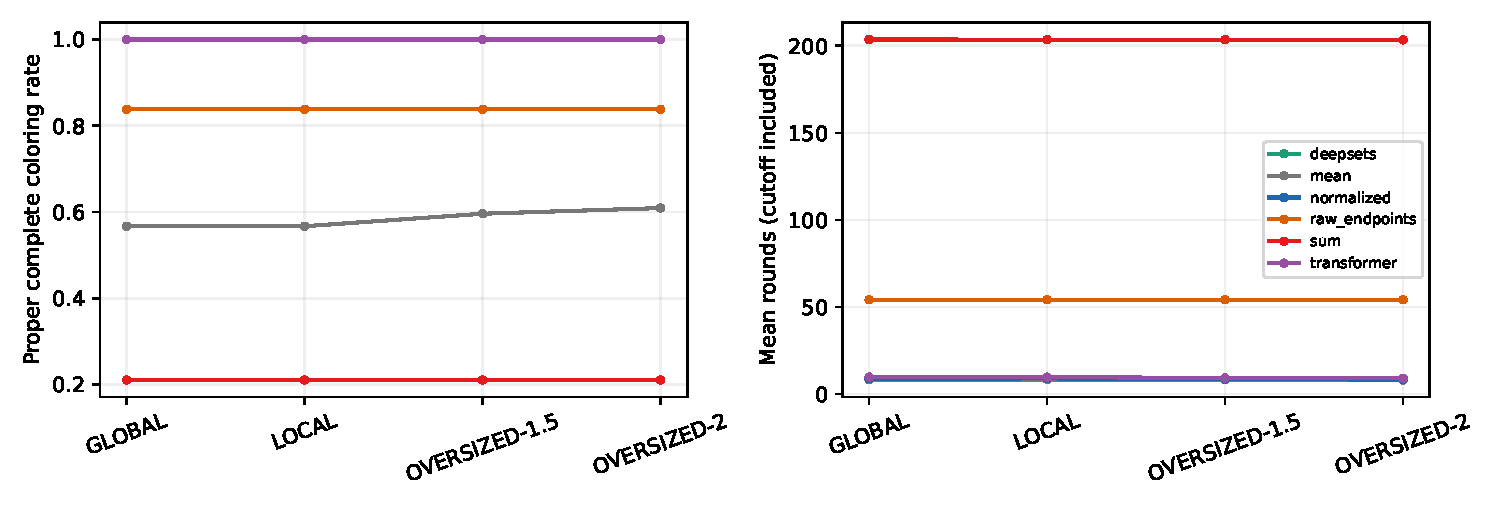
\includegraphics[width=\linewidth]{figures/local-palette-outcomes.pdf}
\caption{Success and capped rounds for the new palette regimes. Comparisons
are paired by graph and private random tape.}\end{figure}}{}

\section{Statistical Distinguishability of Learned Coloring Policies}
\label{sec:statistical-laws}
Successful coloring does not require exact teacher imitation. To characterize
what was learned, fix the \emph{same} local state $S$ before comparing policies.
The observer knows $S$, the list and the available set, observes IID candidate
colors, and does not observe random draws, logits or internal activations.
This differs from identifying models from their autonomously visited states.

\paragraph{Three distinct comparisons.}
Shared-randomness fidelity is
$F_M(S)=\Pr[f_M(S,r_c)=f_L(S,r_c)]$. Candidate-law comparison instead concerns
$q_M(c\mid S)=\Pr[f_M(S,r_c)=c]$ and the uniform teacher law on $A_v$.
For finite-sample identification, the hypotheses are $q_L^m$ versus $q_M^m$.
Participation, candidates conditional on participation, and final confirmed
colors must not be pooled. In these actual implementations participation sees
only $(r_p,u_v)$ and the candidate pathway sees $r_c$ and deterministic state,
so private independent draws imply conditional independence. COMMIT and
confirmation additionally depend on neighboring offers.

\begin{proposition}[Fidelity need not determine a candidate law]
For any state with $k\ge2$ available colors there exist two candidate maps
with zero shared-r fidelity and identical uniform candidate laws.
\end{proposition}
\begin{proof}
For sorted colors $a_0,\ldots,a_{k-1}$ take
$f_L(r)=a_{\lfloor kr\rfloor}$ and
$f_M(r)=a_{(\lfloor kr\rfloor+1)\bmod k}$. They disagree everywhere on $[0,1)$,
and each color has a preimage of length $1/k$ for either map.
\end{proof}
Consequently no candidate-only classifier can distinguish these two laws at
this state, regardless of sample size. Their equality at one state does not
establish equality over every reachable state.

\paragraph{Transition-law equivalence.}
If policies share the conditional \emph{joint} law of all relevant actions at
every state and use the same update function, their next-state laws are the
same pushforward of that action law. With identical initialization, induction
then gives identical trajectory laws. Equality of candidate marginals alone
does not suffice: two adjacent always-participating nodes with identical
shared uniform candidates always collide, whereas independent uniform binary
candidates collide with probability $1/2$. Coupling participation to the
candidate can likewise change transition laws without changing either marginal.

\paragraph{Distances and optimal classification.}
For known laws $P,Q$ and equal priors, optimal balanced accuracy is
$(1+\operatorname{TV}(P^m,Q^m))/2$: choosing $Q$ on event $D$ yields accuracy
$1/2+(Q^m(D)-P^m(D))/2$, maximized by the likelihood-ratio event. Writing
$\delta=\operatorname{TV}(P,Q)$ and $\rho=\sum_c\sqrt{P(c)Q(c)}$, we use
\[
\max\{\delta,1-\rho^m\}\le\operatorname{TV}(P^m,Q^m)
\le\min\{1-(1-\delta)^m,\sqrt{1-\rho^{2m}}\}.
\]
The first upper bound follows by independent maximal couplings; the affinity
factorizes, giving the Hellinger bounds by Cauchy--Schwarz. The lower bound
$\delta$ follows by projection to one coordinate. These are exact inequalities
for known laws, not certificates obtained by inserting uncertain estimates.

\paragraph{Sampling and uncertainty.}
The prespecified states use $K=4,11,51,101,201,501$, with all-free, singleton,
two/three-color, contiguous, alternating and scattered available sets. Legal
local-list witnesses extend high-color fixed neighbors with private pending
leaves. Additional frozen autonomous states retain their generator and graph
provenance and are secondary analyses. Every policy is queried on the same
frozen state. We report deterministic midpoint and boundary probes separately
from IID Monte Carlo; quadrature does not receive binomial intervals.

Each network/state has 32,768 distribution-estimation draws and 8,192
independent shared-r fidelity/test draws. For six prespecified contexts and
all thirty networks, candidate-only likelihood-ratio tests use independent
fresh candidate samples at $m=1,5,20,100,500,2000$, 256 test trials per source,
and 1,024 independent teacher calibration trials. Test trials use nested
prefixes over $m$, so points on a curve are paired. The plug-in alternative
uses pseudocount $1/2$ per palette color: an unobserved category is not
declared impossible. Teacher support is known exactly. Equal-prior accuracy
uses threshold zero with randomized ties; level-0.05 power uses a separately
calibrated conservative threshold. Neither is an exact Bayes classifier for
an unknown network law.

For $N$ IID draws on $K$ categories, the subset characterization of TV and
Hoeffding's inequality give
$\Pr(\operatorname{TV}(\widehat q,q)\ge\epsilon)
\le2^K\exp(-2N\epsilon^2)$. This provides a conservative pointwise uncertainty
radius for distances from the known teacher law. Approximate equivalence
requires an upper confidence bound at most the prespecified TV tolerance
0.05; failure to reject is not equivalence. We also report JS, Hellinger,
entropy, inverse collision probability, largest mass, forbidden mass and
shared-r rank error, before aggregation by network/state. Float64 teacher
inputs and clipped float32 model inputs are compared explicitly at boundaries.

\IfFileExists{tables/distribution-results-prose.tex}{For all-free $K=201$, normalized had mean estimated TV 0.046, shared-r fidelity 0.053, and 194.6 effective colors (inverse collision probability). For all-free $K=201$, deepsets had mean estimated TV 0.164, shared-r fidelity 0.021, and 63.2 effective colors (inverse collision probability). For all-free $K=201$, transformer had mean estimated TV 0.291, shared-r fidelity 0.020, and 23.7 effective colors (inverse collision probability). For all-free $K=201$, e1-original had mean estimated TV 0.064, shared-r fidelity 0.038, and 173.2 effective colors (inverse collision probability). The original E1 networks are a separate historical cohort, not the new NORMALIZED replicas. Estimation uncertainty and per-state sample-based classification curves are reported separately; low power is not a proof of equality. 
}{
\todo{Awaiting conditional-law estimates and independent classifier test curves.}}
\IfFileExists{figures/candidate-fidelity-and-tv.pdf}{
\begin{figure}[ht]\centering
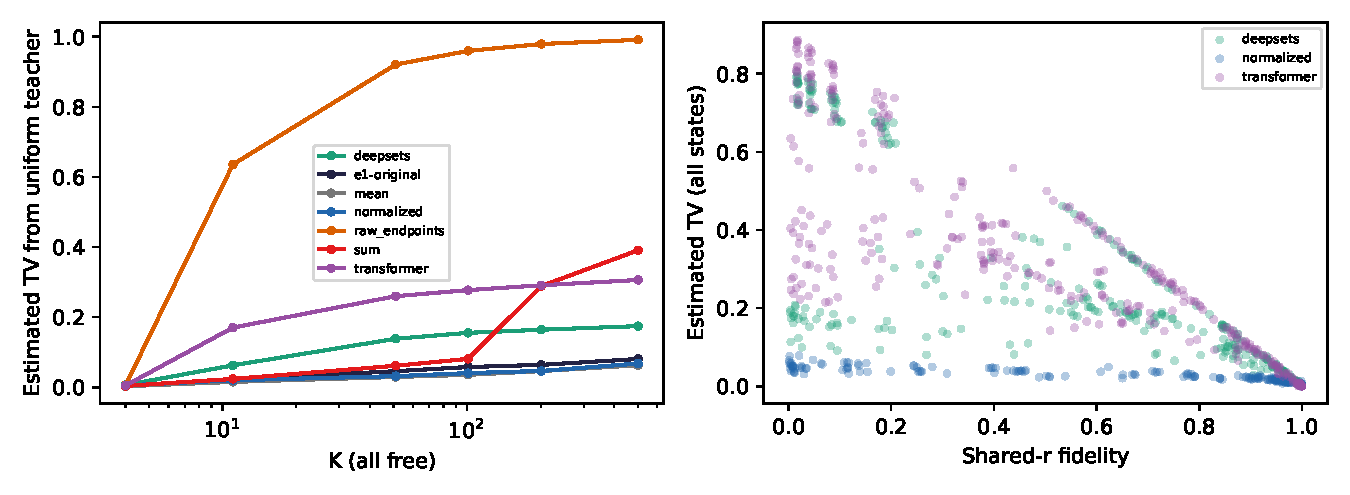
\includegraphics[width=\linewidth]{figures/candidate-fidelity-and-tv.pdf}
\caption{Conditional candidate-law distance versus palette size, and shared-r
fidelity versus law distance. Each point derives from a fixed state; quadrature
and Monte Carlo are stored separately.}\end{figure}}{}
\IfFileExists{figures/candidate-distinguishability.pdf}{
\begin{figure}[ht]\centering
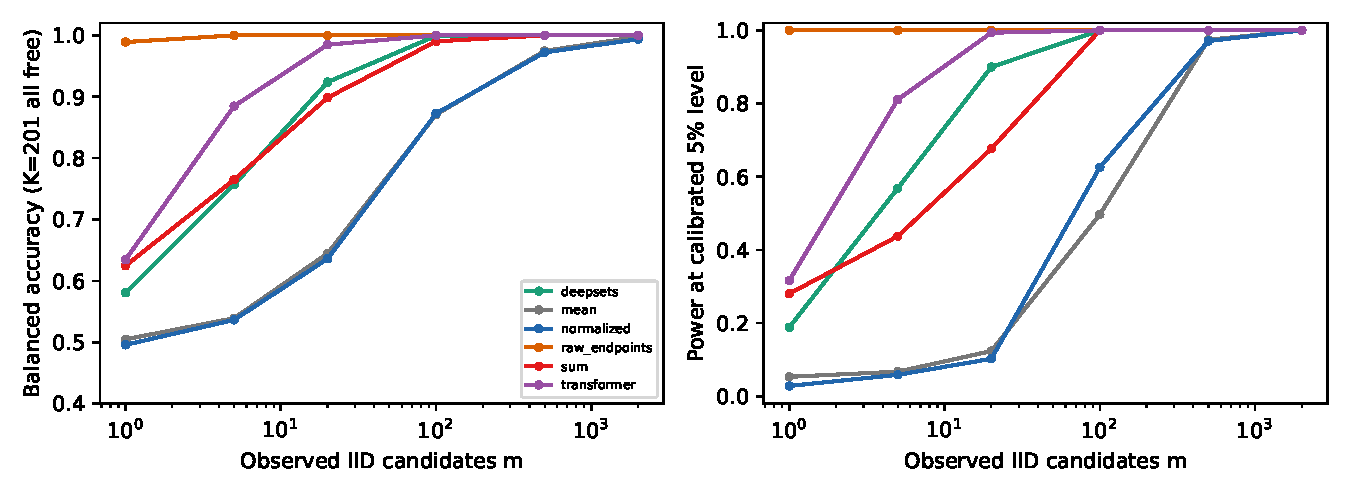
\includegraphics[width=\linewidth]{figures/candidate-distinguishability.pdf}
\caption{Independent candidate-only test performance for all-free $K=201$.
The curves summarize fixed checkpoints, not learned-law Bayes certificates.}
\end{figure}}{}

\paragraph{Distribution and progress.}
For exact COMMIT and conditionally private independent actions, formula~(1) in
the accompanying theory document applies even to heterogeneous lists. A useful
TV perturbation consequence is the following: if $q_v$ is supported on $L_v$,
$\epsilon_v=\operatorname{TV}(q_v,\operatorname{Unif}(A_v))$ and $p_u\le p_{\max}$,
\[
 P_v\ge p_v\max\{0,1-p_{\max}t_v/k_v-\epsilon_v\}.
\]
Indeed the probability of surviving neighbors' offers is a function of the
candidate in $[0,1]$; changing its expectation from uniform costs at most TV.
Thus at $p=1/2$ sufficiently small nonuniformity retains a positive constant
bound, even if statistically detectable. Conversely, deterministic proposals
on an all-free clique have the same one-node TV and entropy whether every
node proposes a common color or different mutually compatible colors; their
confirmation probabilities can be $2^{-K}$ or $1/2$. Marginal distance alone
therefore cannot universally rank speed. The controlled experiments substitute
uniform/learned/mixture candidate laws at the same state and exact COMMIT;
autonomous round-count correlations remain descriptive.
\IfFileExists{tables/progress-results-prose.tex}{normalized, learned-estimated: mean exact-COMMIT probability 0.2994. normalized, half-uniform-mixture: mean exact-COMMIT probability 0.3028. deepsets, learned-estimated: mean exact-COMMIT probability 0.2709. deepsets, half-uniform-mixture: mean exact-COMMIT probability 0.2893. transformer, learned-estimated: mean exact-COMMIT probability 0.2380. transformer, half-uniform-mixture: mean exact-COMMIT probability 0.2758. These are controlled plug-in predictions from estimated laws, with fixed participation 1/2; the heterogeneous-state experiment independently checks one-round confirmations. 
}{
\todo{Awaiting controlled exact-versus-learned COMMIT and mixture interventions.}}
